\chapter{FUNDAMENTAÇÃO TEÓRICA}
\label{chap:fundamentacaoTeorica}

% FUNDAMENTAÇÃO-TEÓRICA-------------------------------------------------------

\section{Sensor Sonar}
\label{sec:sonar}

\subsection{Princípio do Sonar}
\label{sec:principio-sonar}

O sonar é um sensor capaz de calcular a distância de objetos em um meio através de ondas sonoras. O sensor emite um pulso de onda que percorre o meio até colidir em um obstáculo/objeto ou ser absorvido completamente pelo meio. Após colidir, parte da onda é refletida e retorna para o sensor (a origem do pulso) com uma intensidade menor. Ao ser captada pelo sensor, a onda é decomposta em várias partes, onde cada parte é conhecida como \textit{bin}. O conjunto de \textit{bins} que compõe uma onda, é chamado de \textit{beam}, como mostra a Figura \ref{fig:imagem_acustica}.

De maneira geral, o sonar poder ser do tipo passivo ou ativo. O sonar passivo apenas escuta o meio com o intuito de filtrar os sinais sonoros de diferentes objetos do ruído do ambiente. Ao passo que, o sonar ativo tem a capacidade de emitir sinais acústicos e captar o retorno do pulso. O alcance de um pulso de um sonar ativo e a qualidade do sinal\footnote{Quanto maior a qualidade do sinal, maior será o nível de detalhamento e discriminação do alvo e menor será a quantidade de ruído.} retornado está relacionado com a frequência de operação do sensor (Tabela \ref{tab:freq-acustica}).

\begin{figure}[H]
    \centering
    \caption{Representação de um \textit{bin} e um \textit{beam} em uma imagem acústica}
    \label{fig:imagem_acustica}
    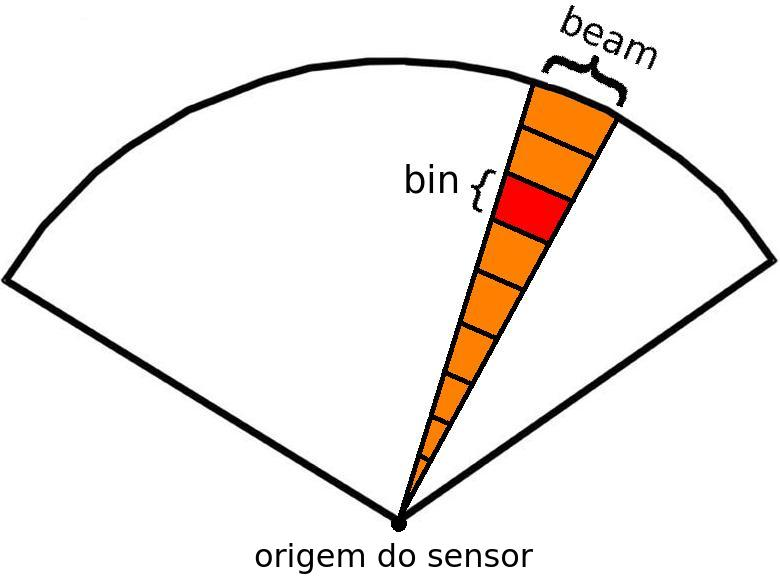
\includegraphics[scale=0.3]{dados/figuras/imagem_acustica.jpg}
\end{figure}

Sinais de alta frequência possuem um curto alcance, porém produz um sinal de retorno que carrega mais informações e com uma alta qualidade. Ao contrário, os sinais de baixa frequência são menos atenuados pelo meio, resultando em uma melhor propagação, mas em compensação, a quantidade de informação no sinal de retorno é menor.

\begin{table}[H]
    \centering
    \caption{Relação entre alcance e frequência da onda acústica}
    \label{tab:freq-acustica}
    \begin{tabular}{@{}lll@{}}
    \toprule
        Frequência & Tamanho da onda & Alcance \\ \midrule
        100 Hz & 15 m & 1000 km ou mais \\
        1 kHz & 1.5 m & 100 km ou mais \\
        10 kHz & 15 cm & 10 km \\
        25 kHz & 6 cm & 3 km \\
        50 kHz & 3 cm & 1 km \\
        100 kHz & 1.5 cm & 600 m \\
        500 kHz & 3 mm & 150 m \\
        1 MHz & 1.5 mm & 50 m \\ \bottomrule
    \end{tabular}
    \fonte{\cite{christ2013rov}}
\end{table}

Sabendo a velocidade de propagação do som no meio e o intervalo de tempo que a onda levou para retornar, é possível calcular a distância do obstáculo até o sensor. 
Definimos como \textit{ping} a ída e retorno de um pulso de som emitido pelo sensor, e tempo de \textit{ping} como o intervalo de tempo para realizar um \textit{ping}. 
A velocidade de propagação do som é maior nos sólidos, pois as moléculas estão mais próximas, transmitindo a energia cinética da onda de umas para as outras com maior facilidade. 
Na Tabela \ref{tab:vel_som}, \cite{halliday2008fundamentals} comprovou esse fato, onde se encontra diferentes velocidades do som de acordo com o meio.

\begin{table}[H]
    \centering
    \begin{threeparttable}
    \caption{Velocidade do som em diferentes meios.}
    \label{tab:vel_som}
    \begin{tabular}{lc}
        \toprule
            \textbf{Meio$^a$} & \textbf{Velocidade (m/s)} \\ 
        \midrule
            \textit{Gases} &  \\
            Ar (0 º C) & 331 \\
            Ar (20 º C) & 343 \\
            Hélio & 965 \\
            Hidrogênio & 1284 \\
            \textit{Líquidos} &  \\
            Água (0 º C) & 1402 \\
            Água (20 º C) & 1482 \\
            Água salgada$^b$ & 1522 \\
            \textit{Sólidos} &  \\
            Aço & 5941 \\
            Alumínio & 6420 \\
            Granito & 6000 \\ \bottomrule
    \end{tabular}
    \begin{tablenotes}
        \item $^a$ A 0 º C e 1 atm de presssão, a menos que haja uma indicação em contrário.
        \item $^b$ A 20 º C e 3,5\% de salinidade.
    \end{tablenotes}
    \end{threeparttable}
    \fonte{\cite{halliday2008fundamentals}.}
\end{table}


\subsection{Sonar \textit{Singlebeam} e \textit{Multibeam}}
\label{sec:single-multibeam}
Além da classificação passiva e ativa, o sonar pode ser agrupado de diversas maneiras, uma delas referente a área de cobertura do sinal.
O sonar \textit{singlebeam} trabalha com apenas um único pulso de onda (Figura \ref{fig:echo-sounder}). Geralmente ele é encontrado na parte inferior dos robôs e posicionado para baixo com o objetivo de encontrar a altitude do robô em relação ao fundo do corpo d'água em que está. Ainda pode ser posicionado nas partes laterais, frontal ou posterior para ser utilizado como um sensor de colisão.

\begin{figure}[H]
    \centering
    \caption{Diferentes modelos de sonares.}
    \label{fig:beams}
    \begin{subfigure}[t]{0.4\textwidth}
        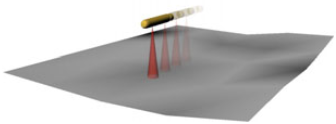
\includegraphics[width=\textwidth]{dados/figuras/singlebeam.png}
        \caption{\textit{Echo sounder.}}
        \label{fig:echo-sounder}
    \end{subfigure}
    \begin{subfigure}[t]{0.4\textwidth}
        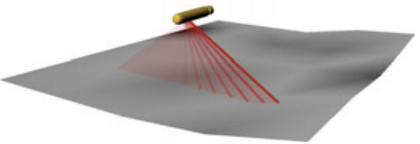
\includegraphics[width=\textwidth]{dados/figuras/mec-scan-profiling.png}
        \caption{\textit{Mechanically scanned profiler.}}
        \label{fig:mec-scan-prof}
    \end{subfigure}
    \begin{subfigure}[t]{0.4\textwidth}
        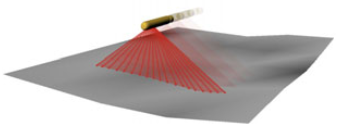
\includegraphics[width=\textwidth]{dados/figuras/multibeam.png}
        \caption{\textit{Multibeam echo sounder.}}
        \label{fig:multi-prof-sonar}
    \end{subfigure}
    \begin{subfigure}[t]{0.4\textwidth}
        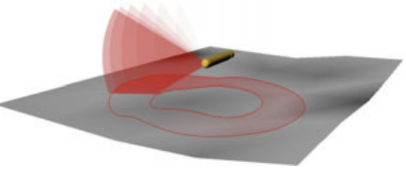
\includegraphics[width=\textwidth]{dados/figuras/msis.png}
        \caption{\textit{Mechanical scanning imaging sonar.}}
        \label{fig:msis}
    \end{subfigure}
    \begin{subfigure}[t]{0.4\textwidth}
        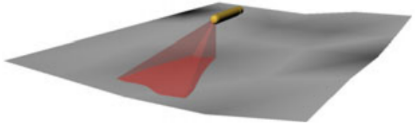
\includegraphics[width=\textwidth]{dados/figuras/fls.png}
        \caption{\textit{Foward looking imaging sonar.}}
        \label{fig:fls}
    \end{subfigure}
    \fonte{Adaptado de \cite{ribas2010underwater}.}
\end{figure}

Por outro lado, o sonar \textit{multibeam} é mais complexo, composto por um conjunto de hidrofones\footnote{Os hidrofones são transdutores de som para eletricidade que captam vibrações sonoras transmitidas no meio, reconhecendo na forma de frequência. Após reconhecer a frequência, o dispositivo transforma em um sinal elétrico.} que emitem vários pulsos de onda de forma simultânea, que juntos possuem o formato de um leque (Figuras \ref{fig:multi-prof-sonar} e \ref{fig:fls}). Esse tipo de sonar é comumente utilizado para fazer batimetria e imageamento de ambientes e superfícies submersas por possuir uma alta qualidade e velocidade de coleta de dados.

\subsection{Sonar MSIS}
\label{sec:msis}
O MSIS (do inglês \textit{Mechanical Scanning Image Sonar}) é um sonar mecânico \textit{singlebeam} de varredura de 360º, ou seja, possui um atuador no cabeçote do sensor para poder girar a partir de passos pré-definidos e imagear o ambiente em seu entorno, ilustrado na Figura \ref{fig:msis}. 
O sensor realiza o escaneamento no plano horizontal, onde o cabeçote gira em um incremento de um ângulo pré-estabelecido, efetuando uma leitura para cada incremento, como mostra a Figura \ref{fig:msis-scanning}.
Para exemplificar, na Figura \ref{fig:msis-image}, apresenta uma imagem de satélite de uma doca com a sobreposição de uma imagem acústica obtida com um MSIS.

\begin{figure}[H]
    \centering
    \caption{Imagem acústica sobreposta em uma imagem de satélite.}
    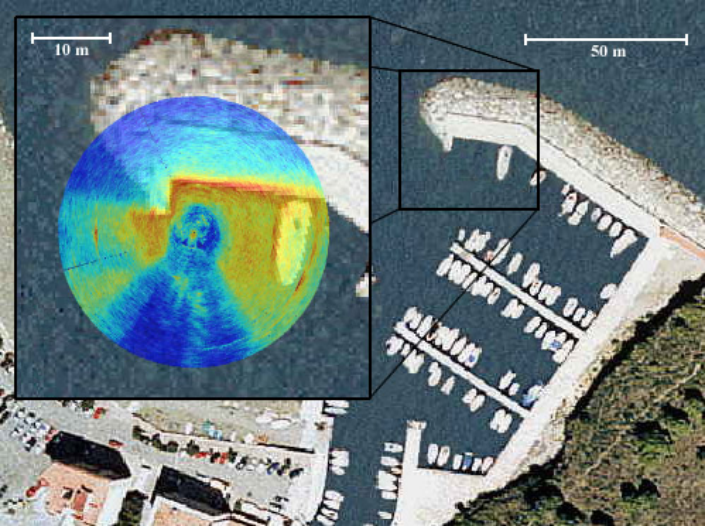
\includegraphics[scale=0.3]{dados/figuras/msis_image.png}
    \fonte{\cite{ribas2006slam}}
    \label{fig:msis-image}
\end{figure}

\begin{figure}[H]
    \centering
    \caption{Representação do processo de escaneamento de um MSIS.}
    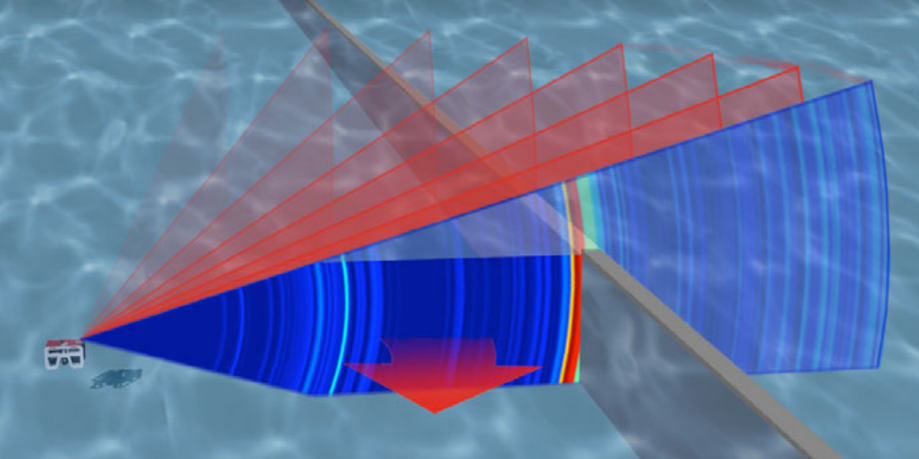
\includegraphics[scale=0.3]{dados/figuras/msis-scanning.png}
    \fonte{\cite{ribas2010underwater}}
    \label{fig:msis-scanning}
\end{figure}

O processo de escaneamento pode ser vagaroso por conta do transdutor rotar os 360 graus\footnote{Geralmente o equipamento possibilita a configuração para um range angular menor do que 360º, tornando menor o tempo de leitura de uma imagem completa.}, porém seu baixo custo e peso torna o modelo viável para aplicações com alto risco de perda do equipamento como no caso das geleiras.

%Precisa falar dos problemas com o MSIS (shadows, imagens distorcidas, ambiguidades, etc..)

\section{\textit{Robot Operating System}}
\label{sec:ros}

O ROS (Sistema Operacional de Robôs, do inglês \textit{Robot Operating System}) é uma plataforma de desenvolvimento de softwares (\textit{framework}) de código aberto direcionado para a área da robótica, que fornece a funcionalidade de um meta-sistema operacional, tais como, abstração de hardware, gerenciamento de pacotes, controle de dispositivos de baixo nível e troca de mensagens entre processos. 
O ROS atua como um \textit{middleware} de comunicação entre aplicações robóticas e o \textit{hardware}, oferecendo ferramentas e bibliotecas para auxiliar no desenvolvimento e execução de aplicações robóticas distribuídas. Os conjuntos de processos em execução do ROS são representados através de uma arquitetura de grafos orientados ou grafos de computação.

\subsection{Grafos de computação}

No ROS, os grafos de computação possui a finalidade de representar sua rede de comunicação P2P entre os processos. O grafo computacional é composto pelos seguintes elementos:

\begin{itemize}
    \addtolength{\itemindent}{2em}
    \setlength\itemsep{1em}
    
    \item Nodos: Os nodos são os processos em execução no sistema e são responsáveis por realizar funções computacionais.  Em um sistema ROS pode haver vários nodos responsáveis por controlar apenas um único robô, como por exemplo, um nodo responsável por controlar a localização do robô, outro nodo controla o sensor laser, outro faz o planejamento da rota, entre outros;
    
    \item Mensagens: As mensagens são estruturas de dados que podem incluir diversos tipos de dados, como inteiros, boleanos, strings, etc. Através das trocas de mensagens, os nodos fazem a comunicação entre si;
    
    \item Tópicos: Os tópicos são canais de comunicação que adotam a semântica de publicação/inscrição de mensagens. Os nodos utilizam essa semântica para publicar mensagens e/ou se inscreverem nos tópicos. Portanto, se um nodo publicar mensagens em um determinado tópico, todos os os nodos inscritos nesse tópico receberão as mensagens. Além disso, podem haver múltiplos nodos inscritos e/ou publicando em um mesmo tópico, assim como um nodo pode publicar e se inscrever em múltiplos tópicos. A Figura \ref{fig:topic_node} ilustra a relação entre nodo e tópico;
    
    \item Serviços: Diferente dos tópicos, os serviços possibilitam uma comunicação direta entre processos, através de interações requisição/resposta que é comumente empregado em sistemas distribuídos;
    
    \item \textit{Bags}: O \textit{bag} é um formato de arquivo usado pelo ROS para gravar e reproduzir dados gerados em um procedimento. Eles são extremamente importantes, pois proporcionam ao usuário gravar dados de sensores e atuadores para poder reproduzir futuramente;
    
    \item \textit{Master}: O \textit{master} permite que os nodos localizem uns aos outros para trocar mensagens ou invocar serviços. Uma vez que os nodos se localizaram através de consultas ao \textit{master}, uma comunicação direta P2P entre os nodos é estabelecida. Além disso, ele tem a tarefa de registrar nodos, tópicos, serviços e parâmetros da rede;
    
    \item Servidor de parâmetros: O servidor de parâmetros faz parte do \textit{master}. Ele é responsável por permitir o compartilhamento distribuído de parâmetros em tempo de execução aos nodos.
\end{itemize}
\hspace{1em}

\begin{figure}[H]
    \centering
    \caption{Relação entre tópico e nodo.}
    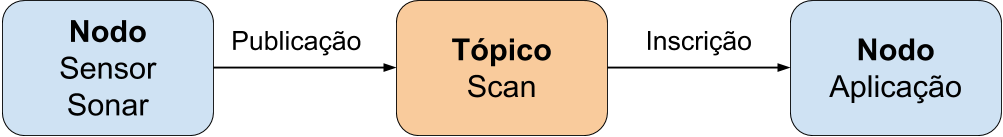
\includegraphics[scale=0.3]{dados/figuras/topic_node.png}
    \label{fig:topic_node}
\end{figure}

A Figura \ref{fig:topic_node} ilustra com um exemplo, o funcionamento da estrutura de tópicos e nodos do ROS. O nodo \textit{Sensor Sonar} é responsável por aquirir os dados da coleta e publicar esses dados no tópico \textit{Scan}. Já o nodo \textit{Aplicação} recebe os dados do tópico \textit{Scan} e com base nesses dados realiza ações, como por exemplo, evitar uma colisão do robô com objetos no ambiente.

\section{Simulador Gazebo}
\label{sec:gazebo}

O Gazebo é um robusto \textit{software} de código aberto para simulação de ambientes virtuais 3D para robôs. O simulador possui uma excelente ferramenta de simulação física, gráficos de alta qualidade, interface gráfica, ferramentas de criação de cenários realísticos e robôs, entre outras qualidades. Além disso, o \textit{software} é integrado com o ROS, colaborando para o desenvolvimento de algoritmos, componentes, dispositivos e resoluções de problemas na área da robótica. A interface gráfica é acessível e intuitiva para o usuário, permitindo manipular o ambiente e seus elementos de forma fácil, como ilustra a Figura \ref{fig:gazebo}. Porém, a simulação em ambientes submersos ainda não está próximo do real, pois a ferramenta ainda não é capaz de adicionar uma das principais características contida no meio subaquático e fundamental para o desenvolvimento da área da visão subaquática, a turbidez na água. 

\begin{figure}[H]
    \centering
    \caption{Interface gráfica do simulador Gazebo}
    \label{fig:gazebo}
    \begin{subfigure}[t]{0.45\textwidth}
        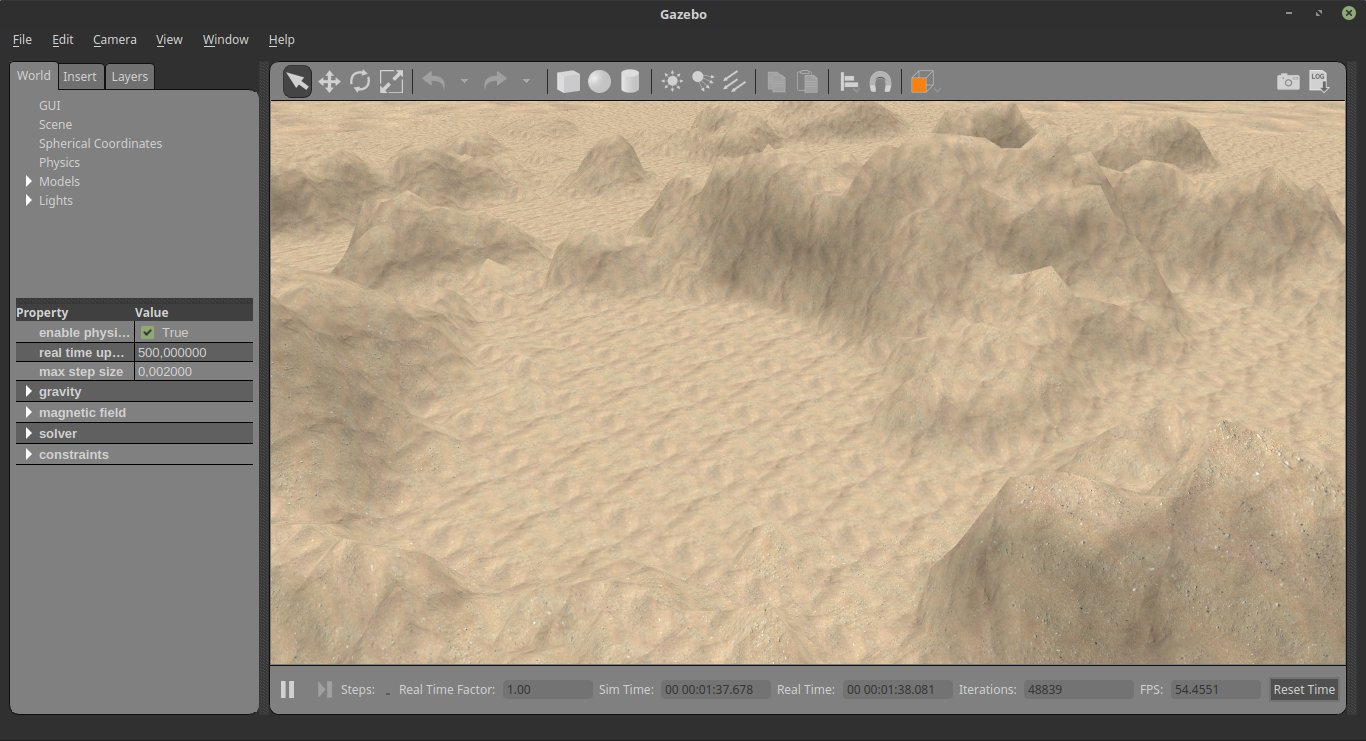
\includegraphics[width=\textwidth]{dados/figuras/gazebo1.jpeg}
    \end{subfigure}
    \begin{subfigure}[t]{0.45\textwidth}
        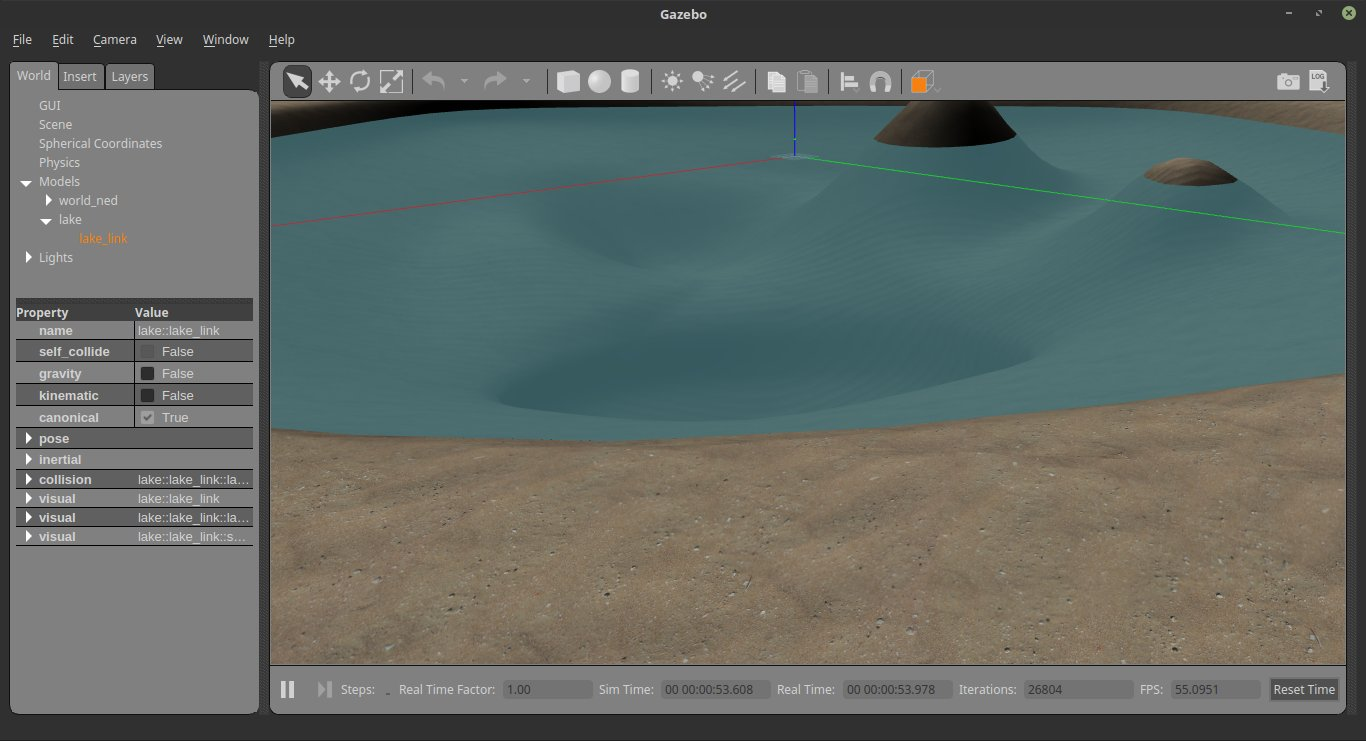
\includegraphics[width=\textwidth]{dados/figuras/gazebo2.jpeg}
    \end{subfigure}
    \begin{subfigure}[t]{0.45\textwidth}
        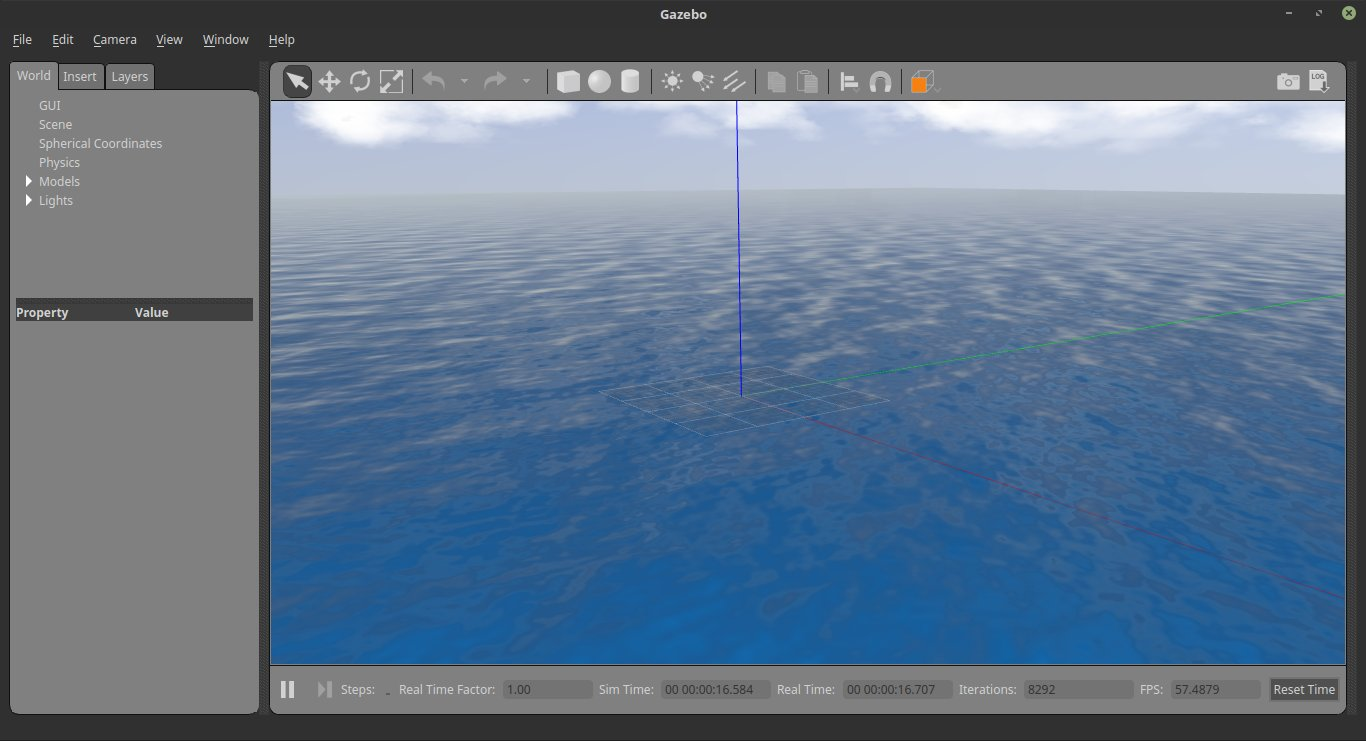
\includegraphics[width=\textwidth]{dados/figuras/gazebo3.jpeg}
    \end{subfigure}
    \begin{subfigure}[t]{0.45\textwidth}
        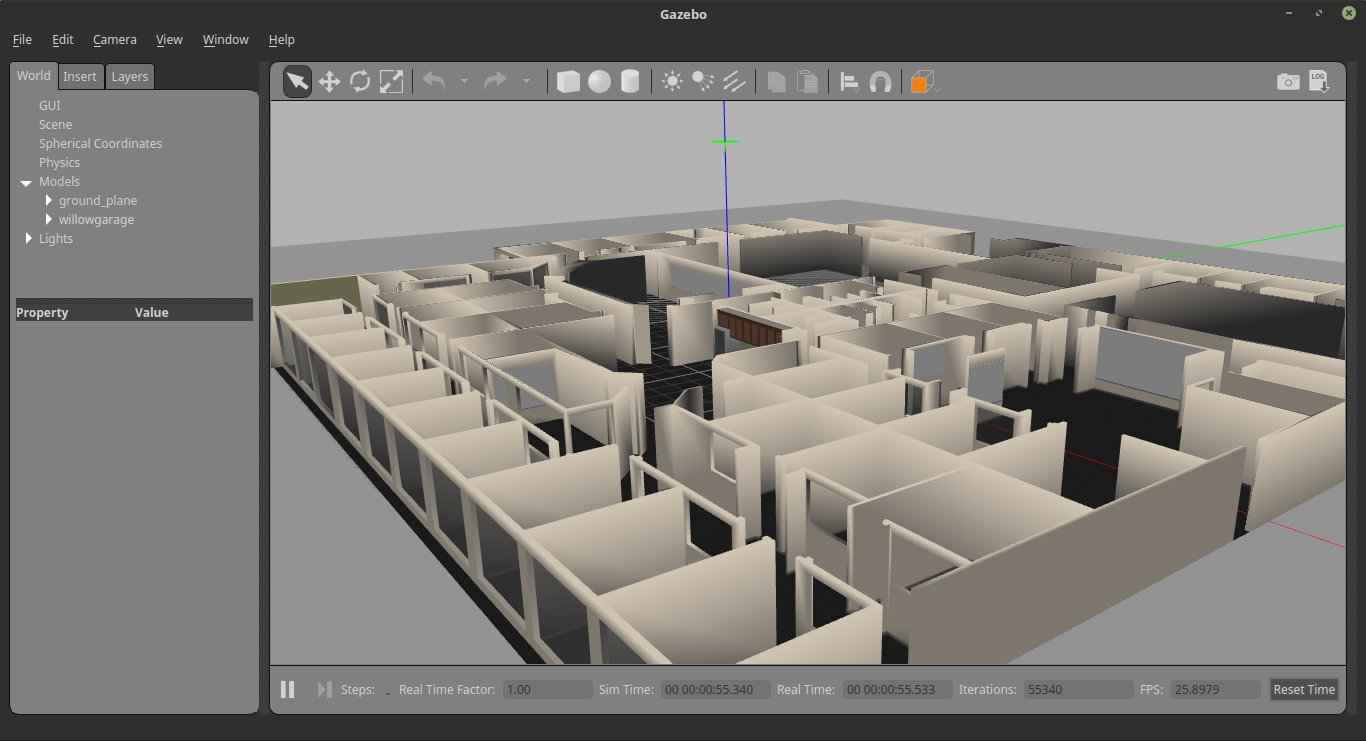
\includegraphics[width=\textwidth]{dados/figuras/gazebo4.jpeg}
    \end{subfigure}
\end{figure}

Contudo, o desenvolvimento em código aberto facilita a criação de pacotes com plugins que auxiliam na simulação, como os pacotes \textit{UUV Simulator} e o Simulador Netuno, desenvolvido por, respectivamente, \cite{manhaes2016uuv} e \cite{longaray2017}. Ambos trabalhos contribuíram para a expansão da área da robótica subaquática.

\section{\textit{GPU Sonar Simulatior}}
\label{sec:gpu_sonar_sim}

O \textit{GPU Sonar Simulator} é um simulador baseado no método proposto por \cite{cerqueira2016gpu}, que utiliza \textit{shaders} para processar imagens de sonar MSIS e FLS com baixo custo computacional. 
Os \textit{shaders} são um conjunto de instruções que definem o comportamento da superfície dos objetos em um processamento gráfico.
Eles são executados na GPU do computador, que é o processador dedicado especialmente para a renderização de gráficos em tempo real. 
Seu funcionamento é determinado pelo \textit{pixel pipeline} ou \textit{pipeline} de renderização 3D, que é a unidade encarregada pela transferência de dados referentes aos pixels que formam uma imagem. 
Portanto, o \textit{pipeline} de renderização 3D é exclusivamente processado na GPU, resultando em uma redução na utilização de recursos da CPU e acelerando o processamento gráfico do computador. 

O simulador foi inicialmente criado para a plataforma ROCK\footnote{O ROCK é um \textit{framework} para o desenvolvimento de sistemas robóticos, semelhante ao ROS. Saiba mais em: \url{https://www.rock-robotics.org/}} (do inglês \textit{Robot Construction Kit}), porém através do trabalho de \cite{longaray2017} foi realizada a adaptação para o ROS.
No desenvolvimento foi utilizado a linguagem \textit{C++} e a ferramenta OSG\footnote{O OSG é um conjunto de ferramentas gráficas 3D de alta performance de código livre e desenvolvida na linguagem \textit{C/C++}. Saiba mais em: \url{http://www.openscenegraph.org/}} (do inglês \textit{Open Scene Graph}).
Quando um ambiente é renderizado no OSG, o \textit{shader} computa dados em um processamento a partir de uma câmera inserida na cena, onde tais dados são divididos em três categorias: 

\begin{itemize}
    \item Intensidade: simula a energia acústica refletida do objeto baseado no ângulo da superfície de contato;
    \item Profundidade: retrata a distância euclidiana entre o ponto central da câmera e o ponto da superfície de contato do obstáculo;
    \item Distorção angular: representa o ângulo entre a coluna central e as colunas nas extremidades da câmera.
\end{itemize}

A intensidade é calculada de acordo com os canais azul e verde, que representam, respectivamente, a intensidade e a distância, como mostra a Figura \ref{fig:shader_output}. Quanto mais claro é o azul em um determinado ponto, maior é a intensidade da energia acústica refletida, ao passo que quanto mais claro for o verde, maior é a distância ou profundidade do sensor até o ponto.

\begin{figure}[H]
    \centering
    \caption{Imagens correspondentes geradas pelo \textit{GPU Sonar Simulator}}
    \label{fig:shader_output}
    \begin{subfigure}[t]{0.5\textwidth}
        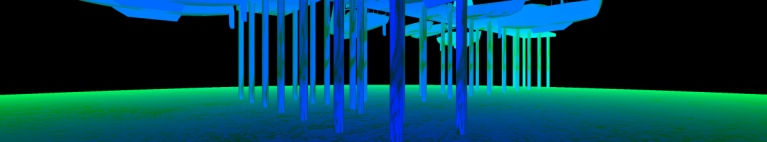
\includegraphics[width=\textwidth]{dados/figuras/shader_output1.png}
        \caption{Imagem gerada pelo \textit{shader}}
    \end{subfigure}
    \begin{subfigure}[t]{0.5\textwidth}
        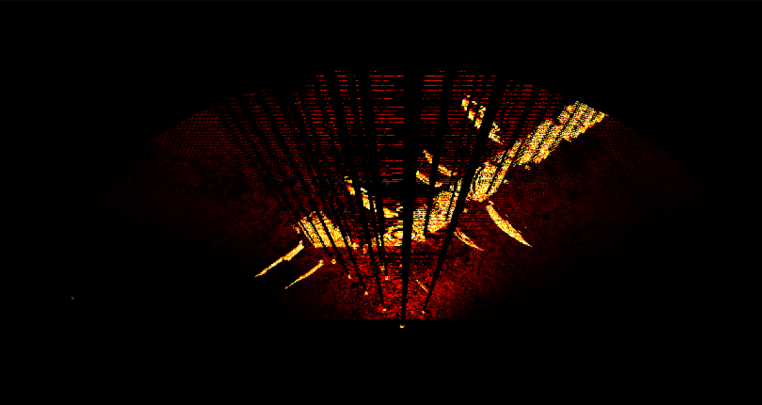
\includegraphics[width=\textwidth]{dados/figuras/shader_output2.png}
        \caption{Imagem acústica resultante.}
    \end{subfigure}
    \fonte{Adaptado de \cite{longaray2017}.}
\end{figure}

O simulador do sonar possui alguns parâmetros de simulação que são definidos pelo usuário, tais como:

\begin{itemize}
    \item Quantidade de \textit{beams}: Define o número de colunas que a imagem será dividida. Se esse parâmetro for igual a 1, então, o simulador executará o sonar MSIS, se for maior que 1, então executará o FLS;
    \item Quantidade de \textit{bins}: Quantidade de valores presentes em um \textit{beam};
    \item \textit{Beam width}: Representa o ângulo de abertura horizontal da observação;
    \item \textit{Beam height}: Representa o ângulo de abertura vertical da observação;
    \item \textit{Range}: Define a distância máxima a ser observado (o alcance do sinal do sonar).
\end{itemize}
\hspace{1em}

\begin{figure}[H]
    \centering
    \caption{Descrição gráfica do método utilizado no simulador do sonar}
    \label{fig:gpu_sonar_sim}
    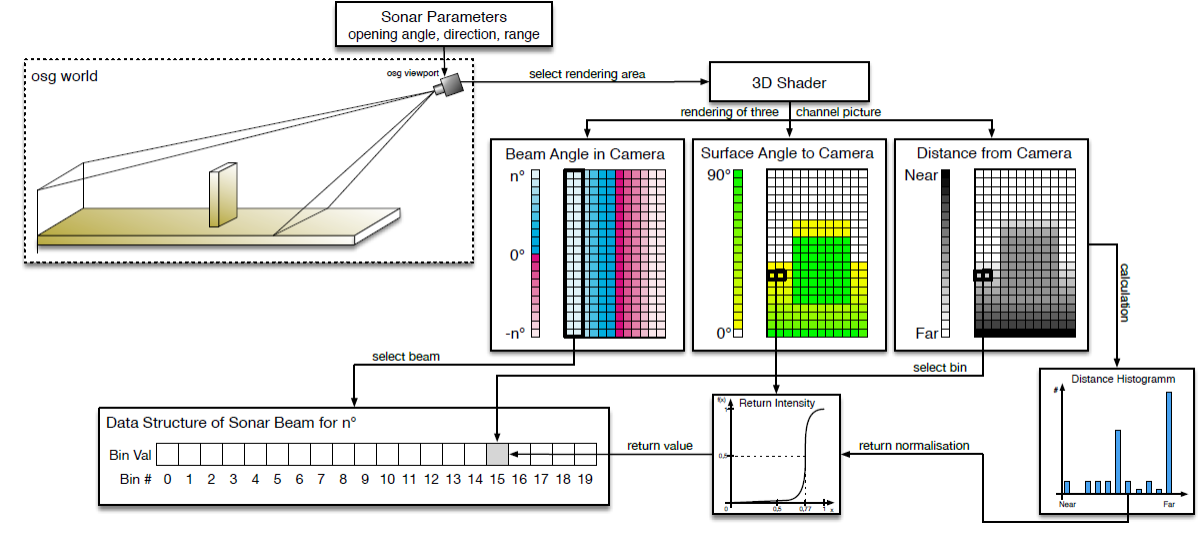
\includegraphics[scale=0.35]{dados/figuras/gpu_sonar.png}
    \fonte{\cite{cerqueira2016gpu}.}
\end{figure}

Esses parâmetros afetam no processamento do simulador e resolução da imagem. Quanto maior o número de \textit{bins}, melhor será a qualidade da imagem acústica. A Figura \ref{fig:gpu_sonar_sim} ilustra o método utilizado no simulador e descrito nessa seção.

\section{\textit{Point Cloud Library}}
\label{sec:pcl}

A PCL (Biblioteca de Nuvem de Pontos, do inglês \textit{Point Cloud Library}) é um \textit{framework} para o processamento de imagens e nuvens de pontos em 2D/3D desenvolvido para a linguagem \textit{C++}. 
O \textit{framework} é um projeto de código aberto em larga escala criado por \cite{rusu2011pcl}. 
A PCL contém diversos algoritmos no estado da arte, incluindo filtros, estimação de \textit{features}, reconstrução de superfícies, segmentação, entre outros. 
Em paralelo, \cite{strawlab2012} adaptou parte da PCL para a linguagem python. 

\begin{figure}[H]
    \centering
    \caption{Exemplo de utilização da PCL em dados adquiridos por um sensor a laser.}
    \label{fig:pcl_example}
    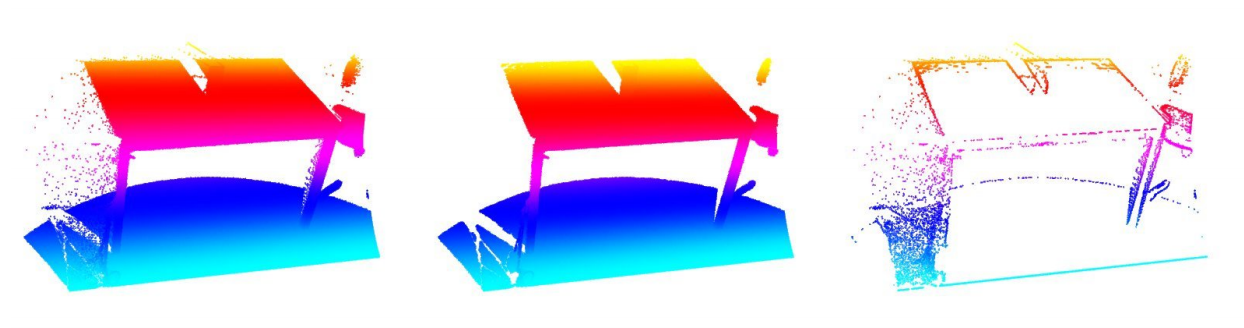
\includegraphics[scale=0.3]{dados/figuras/pcl_example.png}
    \fonte{\cite{rusu2011pcl}.}
\end{figure}

A Figura \ref{fig:pcl_example} ilustra um exemplo da aplicação da PCL em uma nuvem de pontos. Na imagem a esquerda mostra uma nuvem de pontos adquirida a partir de um sensor a laser, a imagem do meio mostra a nuvem resultante após passar por um filtro\footnote{O filtro utilizado se chama \textit{StatisticalOutlierRemoval} (filtro estatístico de remoção de \textit{outliers}) descrito na Seção \ref{sec:statistical_outlier_removal}. A documentação do filtro se encontra em: \url{http://pointclouds.org/documentation/tutorials/statistical_outlier.php}.}, por último, os pontos descartados são mostrados na figura na direita.